\documentclass[12pt]{article}
\usepackage[left=1in, right=1in, bottom=1in, top=1.5in]{geometry}
\usepackage{amsmath}
\usepackage{amsfonts}
\usepackage{amsthm}
\usepackage{amssymb}
\usepackage{epsfig}
\usepackage[colorlinks=true,urlcolor=blue,linkcolor=blue]{hyperref}
\usepackage{amscd}
\usepackage{xcolor}
\usepackage{enumerate}
\usepackage[T1]{fontenc}
\usepackage[toc]{appendix}
\usepackage{mathrsfs}
\usepackage{tensor}     % index positioning in tensor componentes: \tensor{M}{^a_b^c_d}
\usepackage{multirow}
\usepackage{fancyhdr} 
\usepackage[numbers, sort&compress]{natbib} %For compressed multicites

%% Definitions
% Comands
\def\be{\begin{equation}}
\def\ee{\end{equation}}

% Functions
\def\arcsinh{{\rm arcsinh}}
\def\sign{{\rm sign}}
\def\min{{\rm min}}

% Expressions
\def\e{e}
\def\ehat{\hat{\text{\textbf{\textit{e}}}}}
\def\ihat{\hat{\boldsymbol{\imath}}}
\def\jhat{\hat{\boldsymbol{\jmath}}}
\def\khat{\hat{\text{\textbf{\textit{k}}}}}
\def\Sinh{{\rm sinh}}  %To avoid the small space between the function and the argument
\def\Cosh{{\rm cosh}}
\def\wfs{\mbi{\omega}_{\rm FS}}
\def\Fermi{\mathscr{F}}
\def\Obs{\mathscr{O}}

%% Operators  %NOTA: ACORDARSE DE MODIFICAR ESTO AL COPIAR Y PEGAR DE LA VERSIÓN LOCAL
\def\crossu{\!\times_{u}\!}
\def\nablau{\nabla\!_u}

%% New commands
\newcommand{\rob}[1]{\left(#1\right)}    % Round brackets
\newcommand{\sqb}[1]{\left[#1\right]}    % Square brackets
\newcommand{\mb}[1]{\mathbf{#1}}         % Math bold face
\newcommand{\cub}[1]{\left\{#1\right\}}  % Curly brackets
\newcommand{\abb}[1]{\left|#1\right|}    % Absolute value brackets
\newcommand{\angb}[1]{\left<#1\right>}   % Angular brackets
\newcommand{\mbi}[1]{\boldsymbol{#1}}    % Math bold and math italic face 
\newcommand{\mc}[1]{\mathcal{#1}}        % \mathcal
\newcommand{\partd}[2]{\frac{\partial #1}{\partial #2}}   % Partial derivative
\newcommand{\A}[1]{\bf A#1}              % Activities of Methdology

\newcommand{\dd}[1]{{\rm d} #1}
\newcommand{\tprod}[2]{{\rm d}#1 \otimes {\rm d} #2}

%% Rewrited commands
\renewcommand{\Re}{\mathbb{R}}           % Real numbers

\voffset = -0.25in
\textheight = 8.0in
\textwidth = 6.5in
\oddsidemargin = 0.in
\headheight = 20pt
\headwidth = 6.5in
\renewcommand{\headrulewidth}{0.5pt}
\renewcommand{\footrulewidth}{0,5pt}

\begin{document}
\thispagestyle{empty}
\begin{center}
	\Large{\bf Gyroscopic precession in the spacetime of the $q$-metric} \\
	\vspace{1.7cm}
	
	{\large Juan Andrés Guarín Rojas}\\
	{\large BSc.}
	\vspace{1.7cm}

	{\large \bf Research proposal to qualify for the degree of}\\
	{\large Magister in Physics} \\
	\vspace{1.7cm}

	{\large Supervisor:} \\
	{\large Antonio Calixto Gutiérrez Piñeres,  
         BSc., M.Sc., Ph.D.}\\
	{\large Universidad Industrial de Santander}
	\vspace{1.6cm}

	{\large Co-supervisor:} \\
	{\large Abraão Jesse Capistrano, 
	 BSc., M.Sc., Ph.D.}\\
	{\large Universidade Federal do Paran\'{a}, Brasil}
	\vspace{1.6cm}

	\vfill
	{\large Universidad Industrial de Santander}\\
	{\large Faculty of Sciences}\\
	{\large School of Physics}\\
	{\large Bucaramanga}\\
	{\large 2026}
\end{center}
\newpage

\noindent {\Large \bf ABSTRACT} \\

\vspace{0.1cm}
\noindent {\bf TITLE}: Gyroscopic precession in the spacetime of the $q$-metric \footnote{Thesis proposal.}.\\

\noindent {\bf AUTHOR}: Juan Andrés Guarín Rojas \footnote{School of Physics, Faculty of Sciences, Universidad Industrial de Santander. Supervisor: Antonio Calixto Gutiérrez Piñeres, Ph.D. }.\\

\noindent {\bf KEY WORDS: } Gyroscopic precession, Fermi-Walker derivative, Frenet-Serret tetrad\\ $q$-metric, mass multipoles, curvature eigenvalues\\


\noindent {\bf DESCRIPTION}: 
\noindent In this proposal we ask ourselves: What contribution does the mass quadrupole moment make to the gyroscopic precession in the $q$-metric? It is known that a free gyroscope's spin is Fermi-Walker transported along its worldline. This property leads to the notion of gyroscopic precession, in which a Fermi-Walker transported vector appears to precess with respect to the comoving observer equipped with a laboratory fixed with respect to the Frenet-Serret (FS) tetrad. The angular velocity of rotation is equal to minus the 4-rotation of the FS tetrad $\wfs$. In this formalism, it is proposed to study the effect of the quadrupole deformation of the $q$-metric on the precession frequency of a gyroscope moving along a quasi-Killing trajectory. This trajectory corresponds to a circular helix moving around the $t$-axis. The problem that it is aimed to solve is whether a gyroscope moving around an astrophysical object only needs to know the mass monopole of the object to describe its precession to a certain degree of precision, or if it also needs to know the mass quadrupole. The $q$-metric is chosen because in this metric it is easy to obtain the pure monopole solution by taking $q\to 0$, which corresponds to the Schwarzschild solution. To further characterize the precession in the $q$-metric, it is proposed to compute the precession frequency at the singularity $r=2m$ of the $q$-metric and at other positions of interest related to the extrema of the curvature eigenvalues in concordance with the repulsive gravity radius conjecture proposed by Luongo, Quevedo and Gutiérrez-Piñeres.
\newpage

\tableofcontents
\newpage

%%%%%%%%%%%%%%%%%%%%%%%%%%%%%%%%%%%%%%%%%%%%%%%%%%%%%%%%%%
%%%%%%%%%%%%%%%%%%%%%%%%%%%%%%%%%%%%%%%%%%%%%%%%%%%%%%%%%%
\section{Introduction}
Gyroscopes are instruments designed to detect and measure changes in the orientation of an accelerating observer. They are widely used in ships and aircraft to monitor rotational motion, as well as ascent and descent, depending on the application. Gyroscopes also play a fundamental role in the operation of Global Navigation Satellite Systems (GNSS), ensuring accurate attitude determination and navigation. Consequently, they are indispensable tools for navigation both on Earth's surface and in orbit around our planet.\\

Gyroscopes may also play a crucial role in future interstellar navigation. This naturally raises the question of how their behavior is influenced by spacetime curvature and by the Lorentzian structure of spacetime itself. In the absence of external torques, the spin vector of a gyroscope, which characterizes its rotational state, undergoes Fermi-Walker transport along its worldline \cite{straumann2004general, misner2017gravitation}. To an observer whose laboratory frame is defined with respect to the Frenet-Serret tetrad, the gyroscope's spin generally appears to rotate about a certain axis, giving rise to the phenomenon of gyroscopic precession. The associated precession frequency encodes information about several important relativistic effects, including the geodetic precession, the Lense-Thirring effect (or frame dragging), and the Thomas precession \cite{semerak1996forces}.\\

Consequently, gyroscopes can serve as sensitive probes of relativistic effects such as frame dragging. Despite substantial experimental efforts and increasingly precise measurements \cite{ciufolini2026lares, everitt2011gravity, ciufolini2004confirmation}, establishing the extent to which the predictions of general relativity concerning frame dragging are confirmed by observations remains an active area of research. Additional experiments are therefore essential to further constrain measurement uncertainties. This question is of considerable significance, since it provides a direct test of Einstein’s theory of gravity and its description of spacetime dynamics in the presence of rotating masses.\\

Mass multipole moments are of central importance in gravitational physics because they quantify departures of a mass distribution from spherical symmetry. Since realistic astrophysical objects are generally rotating and deformed, they are expected to possess non-zero multipole moments beyond the mass monopole. These moments provide a progressively more detailed characterization of the gravitational source and its exterior field. Indeed, modeling the spacetime outside compact objects such as neutron stars and white dwarfs often requires the incorporation of higher-order multipoles \cite{quevedo2016quadrupolar}. While the mass dipole moment can be removed by a suitable coordinate choice corresponding to the center-of-mass frame in the Newtonian limit, the mass quadrupole moment represents the first physically meaningful correction to the monopolar gravitational field \cite{quevedo2016quadrupolar}.\\


As a representative example of a spacetime with a non-zero mass quadrupole moment, one may consider the $q$-metric \cite{quevedo2011mass}. This geometry is commonly regarded as the simplest exact vacuum solution of the Einstein field equations that incorporates a quadrupolar mass deformation \cite{quevedo2016quadrupolar, beissen2023gravitational}. The spacetime is static and axially symmetric, with all of its mass multipole moments determined by the quadrupole parameter $q$. Remarkably, only the mass monopole and mass quadrupole are independent, while all higher multipoles are uniquely fixed by these quantities \cite{quevedo2011mass}. In the Schwarzschild limit, $q \to 0$, the quadrupole moment vanishes, and the spacetime reduces to that of a spherically symmetric source. Therefore, for small values of $q$,  the $q$-metric offers a natural setting in which to study perturbative effects arising from quadrupolar deformations, including their influence on gyroscopic precession.\\


As discussed above, one of the most important applications of gyroscopes is spacecraft navigation, particularly for satellites orbiting astrophysical bodies. In this context, a natural question arises: is the mass monopole sufficient to describe gyroscopic precession accurately, or do higher-order multipole moments make a significant contribution? Motivated by this issue, the present work addresses the following question: {\it what is the contribution of the mass quadrupole moment to gyroscopic precession in the $q$-metric? }Since the Schwarzschild spacetime is recovered in the limit $q \to 0$, the $q$-metric provides a convenient framework for isolating the monopolar contribution and identifying the leading-order effects arising from the quadrupole moment. Consequently, investigating gyroscopic precession in this spacetime may offer valuable insight into the broader problem of understanding how quadrupolar mass deformations influence gyroscopic motion in more general gravitational fields.



%%%%%%%%%%%%%%%%%%%%%%%%%%%%%%%%%%%%%%%%%%%%%%%%%%%%%%%%%%
%%%%%%%%%%%%%%%%%%%%%%%%%%%%%%%%%%%%%%%%%%%%%%%%%%%%%%%%%%
\section{Theoretical framework}

\subsection{Notation}
The following conventions and notations are based on those presented in \cite{gourgoulhon2013special, chandrasekhar1998mathematical}.

\begin{center}  \bf Indices \end{center}
%\subsubsection*{Indices}
Latin indices $a,b,c,\dots$ denote components in an arbitrary basis. They run from $0$ to $3$ unless otherwise specified.

\noindent Greek indices $\alpha,\beta,\mu,\dots$ denote components with respect to the local coordinate basis $\{\partial_\mu\}$. They run from $0$ to $3$ unless otherwise specified.

\begin{center} \bf Metric and tetrads \end{center}
%\subsubsection*{Metric and tetrads}
The metric tensor is denoted by $\mbi{g}$, and the inverse metric by $\mbi{g}^{-1}$.

\noindent The signature of the metric is $(-,+,+,+)$.

\noindent The Frenet-Serret tetrad is denoted by $\{\mbi{e}_{(a)}\}$, with tetrad indices written between parentheses. 

\begin{center} \bf Maps induced by the metric \end{center}
%\subsubsection*{Maps induced by the metric}
\noindent The natural isomorphisms between the cotangent and tangent bundles are denoted by $\sharp$ and $\flat$ and are defined by
\begin{align}
	\sharp:T^{*}\!M &\longrightarrow TM \notag \\
	\mbi{\omega} &\longmapsto \mbi{g}^{-1}(\mbi{\omega},\cdot)\equiv\mbi{\omega}^\sharp\,,
	%\mbi{\omega} &\longmapsto \mbi{\omega}^\sharp := \mbi{g}^{-1}(\mbi{\omega},\cdot)\,,
\end{align}
\begin{align}
	\flat: TM &\longrightarrow T^{*}\!M \notag \\
	\mbi{v} &\longmapsto \mbi{g}(\mbi{v},\cdot)\equiv \mbi{v}^\flat\,,
	%\mbi{v} &\longmapsto \mbi{v}^\flat:= \mbi{g}(\mbi{v},\cdot)\,,
\end{align}
where $\mbi{g}(\mbi{v},\cdot)$ is defined as the 1-rank tensor $\mbi{g}(\mbi{v},\cdot):TM\to\Re$, $\mbi{w}\mapsto \mbi{g}(\mbi{v},\mbi{w})$, and analogously for $\mbi{g}^{-1}(\mbi{\omega},\cdot)$. In index notation, the action of these isomorphisms is equivalent to raising or lowering indices with the metric, as in $v_a = g_{ab}v^b$.

%The notations $\mbi{\omega}^\sharp$ and $\mbi{v}^{\flat}$ are used to denote the application of the isomorphisms to the 1-form $\mbi{\omega}$ and the vector $\mbi{v}$, respectively. 

\noindent The dot product associated with the metric is denoted by
\be
	\mbi{u}\cdot \mbi{v} := \mbi{g}(\mbi{u},\mbi{v})\,.
\ee

\noindent The Levi-Civita tensor $\mbi{\epsilon}$ induces a cross product on the orthogonal space $E_u$ to a vector $\mbi{u}$ as
\be	
	\mbi{v},\mbi{w}\in E_u\,, \quad \quad \mbi{v}\crossu \mbi{w}:=\mbi{\epsilon}(\mbi{u},\mbi{v},\mbi{w},\cdot)^{\sharp}\,,
\ee
where $\mbi{v}\in E_u$ if $\mbi u\cdot \mbi{v} = 0$. If $\{\mbi{E}_a\}$ is a right-handed orthonormal basis with $\mbi{E}_0 = \mbi{u}$, one can show that
\be
	\mbi{E}_i\crossu\mbi{E}_j = \mbi{E}_k\,,
\ee
where $i,j,k\in\{1,2,3\}$ are cyclic.

%\be
%	\mbi{E}_i\crossu\mbi{E}_j = \tensor{\varepsilon}{_i_j^k}\mbi{E}_k\,,
%\ee
%where $i,j,k\in\{1,2,3\}$, and where $\tensor{\varepsilon}{_i_j^k}$ are the Levi-Civita symbols, not to be confused with the components $\tensor{\epsilon}{_0_i_j^k}$ of the Levi-Civita tensor.

\begin{center} \bf Derivatives \end{center}
%\subsubsection*{Derivatives}
The covariant derivative of a tensor $\mbi{T}$ in the direction of $\mbi{u}$ is denoted by $\nablau\mbi{T}$\,.

\noindent The Fermi-Walker derivative is defined as
\be
	\Fermi_u\mbi{v} := \nablau \mbi{v} +  (\mbi{u}\cdot\mbi{v})\,\mbi{a} - (\mbi{a}\cdot\mbi{v})\,\mbi{u}\,,
\ee
where $\mbi{a}=\nablau\mbi{u}$. A vector $\mbi{v}$ is Fermi-Walker transported along the integral curves of $\mbi{u}$ if $\Fermi_u\mbi{v}=\mbi{0}$.

\noindent The derivative with respect to an observer $\Obs$ with 4-velocity $\mbi{u}$, equipped with an orthonormal tetrad $\{\mbi{E}_a\}$, with $\mbi{E}_0=\mbi{u}$, is defined as
\be
	D_\Obs\,\mbi{v} := \frac{dv^a}{d\tau}\mbi{E}_a\,,
\ee
where $v^a$ are the components of $\mbi{v}$ in the tetrad's basis $\{\mbi{E}_a\}$, and where $\frac{d}{d\tau}$ is the derivative with respect to the proper time $\tau$ of $\Obs$ defined as
\be
	\frac{df}{d\tau} := \nablau f= u^\mu\, \partial_\mu f\,.
\ee

\subsection{Gyroscope precession}
In Newtonian mechanics, a gyroscope may be regarded as a spinning rigid body with two equal principal moments of inertia and a center of rotation located at its center of mass \cite{goldstein2011classical}. To allow unrestricted changes in orientation, gyroscopes are commonly supported by gimbals that permit rotation about three orthogonal axes. When no external torque acts on the system, the spin axis preserves a constant direction relative to an inertial observer, a phenomenon referred to as gyroscopic inertia. As a result, any apparent variation in the orientation of the spin axis reflects the acceleration or rotation of the observer's frame rather than a change in the gyroscope itself. This principle underlies the widespread use of gyroscopes in navigation systems, where they provide information about a vehicle's attitude and rotational dynamics. \\

In the framework of special relativity, the behavior of a gyroscope differs from its Newtonian counterpart. Even when observed from an inertial frame, the spin axis of a gyroscope moving along an accelerated trajectory generally undergoes a precession known as Thomas precession \cite{jonsson2007gyroscope}. The origin of this effect lies in the Lorentz group structure: successive Lorentz boosts along non-collinear directions do not combine into a single boost but instead produce an additional spatial rotation, called the Thomas rotation \cite{gourgoulhon2013special}. Therefore, whenever a gyroscope follows an accelerated worldline, its spin vector is expected to exhibit Thomas precession as a purely relativistic kinematical effect.


Mathematically, the Fermi-Walker derivative elegantly describes the change in the gyroscope's rotation axis. It is more convenient to work with the gyroscope's intrinsic angular momentum, its spin $\mbi{s}$, which is collinear with the gyroscope's rotation axis. The evolution law for the spin of a system takes the form $\Fermi_u \mbi{s}=\mbi{N}$, where $\Fermi_u$ is the Fermi-Walker derivative relative to the system's 4-velocity $\mbi{u}$, and $\mbi{N}$ is the $4$-torque on the spin \cite{gourgoulhon2013special}. Hence, in a torque-free gyroscope, the spin is Fermi-Walker transported along the gyroscope's worldline. The Fermi-Walker transport encapsulates the Thomas precession experienced by the gyroscope. \\


In general relativity, the dynamic law of the gyroscope's spin $\mbi{s}$ remains the same \cite{straumann2004general}
\be
\Fermi_u \mbi{s}=\mbi{N}\,,
\ee
where $\mbi{u}$ is the gyroscope's $4$-velocity and $\mbi{N}$ is the $4$-torque on the spin, as before. In contrast to the previous case, the affine connection $\nabla$ involved in the definition of $\Fermi_u$ is no longer derived from the Minkowski metric but from a general curved metric $\mbi{g}$. As before, in the absence of torques, the gyroscope's spin is Fermi-Walker transported along its worldline. This transport should include the known precession effects in general relativity: Thomas precession, Lense-Thirring precession (frame-dragging), and geodetic precession \cite{semerak1996forces}.\\

A known identity relates the Fermi-Walker derivative $\Fermi_u$ to the derivative with respect to the observer equipped with the Frenet-Serret tetrad and with 4-velocity $\mbi{u}$, and to the $4$-rotation $\wfs$ of the Frenet-Serret tetrad as \cite{straumann2004general, gourgoulhon2013special}
\be
	\Fermi_u\mbi{v} = D_\Obs\, \mbi{v} + \wfs \crossu \mbi{v}\,.
\ee
Here, $D_\Obs$ corresponds to $D_\Obs\,\mbi{v}=\frac{dv^{(a)}}{d\tau}\mbi{e}_{(a)}$, where $v^{(a)}$ are the components of $\mbi{v}$ in the Frenet-Serret tetrad's base $\{\mbi{e}_{(a)}\}$. If $\mbi{v}$ is Fermi-Walker transported along the integral curves of $\mbi{u}$, then
\be
	D_\Obs\, \mbi{v} = -\wfs \crossu \mbi{v}\,,
\ee
so that $\mbi{v}$ appears to rotate with respect to the observer $\Obs$ with angular velocity $-\wfs$. This leads to the notion of gyroscope precession, in which a free gyroscope's spin appears to rotate with respect to a comoving observer with the gyroscope, which is equipped with a laboratory fixed with respect to the observer's Frenet-Serret tetrad. Such a laboratory can be one in, for example, the walls are kept parallel to the direction of $\mbi{e}_{(1)}$ or $\mbi{e}_{(2)}$ (see Fig. \ref{fig:gyroscope_and_observer}).\\

\begin{figure}[h!]
	\centering
	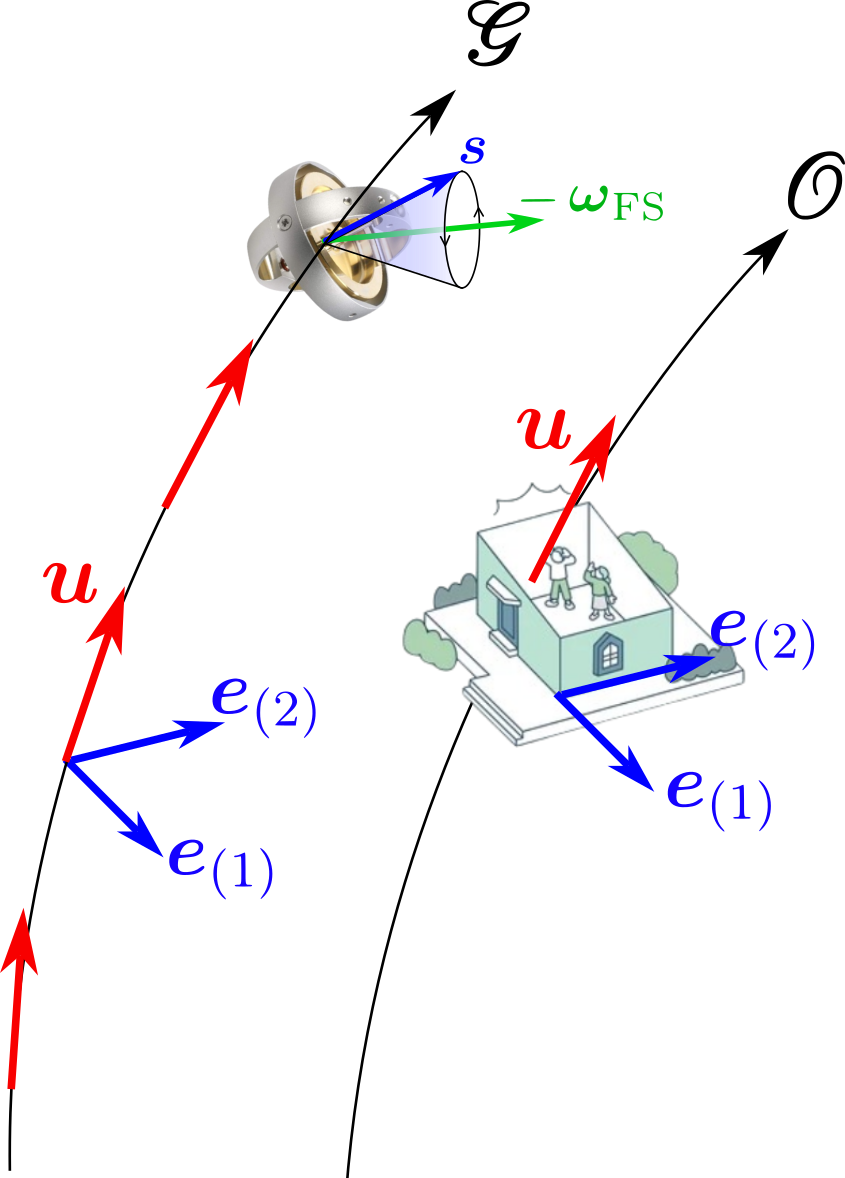
\includegraphics[width=0.4\textwidth]{images/gyroscope_and_observer.png}
	\caption{Schematic representation of an observer $\Obs$ comoving with a free gyroscope $\mathscr{G}$. The gyroscope's spin appears to rotate with respect to a laboratory associated to $\Obs$ whose walls are fixed with respect to the Frenet-Serret tetrad $\{\mbi{e}_{(a)}\}$.}
	\label{fig:gyroscope_and_observer}
\end{figure}

The 4-rotation of the Frenet-Serret tetrad is related to the first and second torsion of the trajectories of $\mbi{u}$ by $\wfs=\tau_1 \mbi{e}_{(3)}+\tau_2\mbi{e}_{(1)}$. The gyroscopic precession frequency is then $\omega_{\rm FS}=\sqrt{\tau_1^2+\tau_2^2}\equiv \Omega_{\rm GP}$. This frequency must depend on the movement of the gyroscope, its 4-velocity and 4-acceleration, on the spacetime's curvature, and on the spacetime's Lorentzian nature \cite{semerak1996forces}. These three sources of precession are present within $\Omega_{\rm GP}$. The contribution of the ``gravitoelectric'' component of the gravitational field, the so-called geodetic precession \cite{semerak1996forces}, can be obtained as a limit case in which the gyroscope moves along a geodesic, as shown in \cite{mukherjee2018horndeski, majumder2025gyroscopic}. However, it is not clear how to obtain the pure contributions of the other sources of precession. Some authors have propose ways to obtain those other contributions based on different formalisms, such as the ones used in \cite{semerak1996forces, mirza2023class}.\\

To study the gyroscope precession, Iyer and Visveshwara \cite{iyer1993frenet} consider gyroscopes moving along ``quasi-Killing'' trajectories. These trajectories are defined by a congruence of observers whose 4-velocity is given by $\mbi{u}=e^{\psi}(\mbi{\xi}+\omega^{A}\mbi{\eta}_{A})$, where $e^{\psi}$ is a normalization factor, $\mbi{\xi}$ is the time-like Killing vector, $\mbi{\eta}_A$, where $A=0,1,\dots$, are the other space-like Killing vectors the spacetime may have, and $\omega^{A}$ are coefficients not necessarily constant. In the case that the $\omega^A$ are constant, the vector $\mbi{\chi}=\mbi{\xi}+\omega^{A}\mbi{\eta}_{A}$ is a Killing vector so that the motion is in the direction of a symmetry of spacetime. In this sense, the given congruence is quasi-Killing, since the coefficients $\omega^A$ are not necessarily constant. In the case that the only other Killing vector to $\mbi{\xi}=\partial_t$ is $\mbi{\eta}=\partial_\phi$, $\omega$ can be interpreted as an angular frequency measured by a distant observer and the congruences $\mbi{u}=e^{\psi}(\partial_t+\omega\partial_\phi)$ are interpreted spatially as circular trajectories around the origin of coordinates.

%An observer equipped with a laboratory fixed with respect to the Frenet-Serret tetrad sees that a free gyroscope's spin rotate with angular velocity $-\wfs$. Such laboratory can be realized, for example, by fixing the walls of the laboratory to the directions of $\mbi{e}_{(1)}$ and $\mbi{e}_{(2)}$.

\subsection{The $q$-metric}
For a stationary axisymmetric spacetime admitting 2-spaces orthogonal to the Killing vectors $\mbi{\xi}=\partial_t$ and $\mbi{\eta}=\partial_\varphi$, the most general metric tensor is the Lewis-Papapetrou \cite{lewis1932some,papapetrou1966champs} metric \cite{stephani2003}
\be
 	 \mbi{g}_{\rm LW} = e^{-2U}(\gamma_{MN}\tprod{x^M}{x^N} + W^2\tprod{\varphi}{\varphi})-e^{2U} (\dd{t}+A\dd\varphi)\otimes (\dd{t}+A\dd\varphi)\,,
\ee
where the functions $U$, $\gamma_{MN}$, $W$ and $A$ depend only on the coordinates $x^M=(x^1,x^2)$ which label the points on the 2-spaces orthogonal to the Killing vectors. If one further assumes that $W$ is a non-constant function, one can find a coordinate transformation in which $W=x^1\equiv \rho$ and
\be
	\mbi{g}_{\rm LW} = e^{-2U}[e^{2k}(\tprod{\rho}{\rho} + \tprod{z}{z}) + \rho^2 \tprod{\varphi}{\varphi}] - e^{2U}(\dd{t}+A\dd\varphi)\otimes (\dd{t}+A\dd\varphi)\,.
\ee
The variables $\rho$ and $z$ are the so called Weyl's canonical coordinates \cite{stephani2003}.\\

If one assumes that $\mbi{\xi}$ is hypersurface-orthogonal, then $A$ can be put equal to zero and the Einstein field equations for vacuum read
\be
	 U\!_{,\rho\rho}+U\!_{,zz}+\frac{1}{\rho}U\!_{,\rho} = 0\,, \quad k_{,\rho}=\rho(U_{,\rho}^2-U_{,z}^2)\,, \quad k_{,z}=2\rho U\!_{,\rho}U\!_{,z}\,,
\ee
where coordinates in the subindices after a comma indicate partial differentiation. These equations are invariant under the Zipoy-Voorhees (ZV) transformation \cite{quevedo2011mass} $U\to U\delta$ and $k\to k\delta^2$, where $\delta$ is a real constant. So that if a solution is known, one gets a new solution by applying this transformation. The solution 
\be
	U=\frac{1}{2} \ln\rob{\frac{r_{+}+r_{-}-2m}{r_{+}+r_{-}+2m}}\,, \quad k=\frac{1}{2}\ln\rob{\frac{(r_{+}+r_{-})^2-4m^2}{4r_{+}r_{-}}}\,,\quad r_{\pm}^2=\rho^2+(z\pm m)^2
\ee
represents the Schwarzschild solution. By implementing the ZV transformation with $\delta=1+q$, one obtains the so called $q$-metric.\\

This solution, parametrized by $q$, has been studied and restudied by many authors \cite{bach1922neue, darmois1927memorial, zipoy1966topology, gautreau1967directional, bonnor1968interpretation, voorhees1970static, esposito1975static,  kodama2003global, quevedo2011mass}. It may seem that the first author to obtain this solution was Rudolf Bach \cite{bach1922neue} in 1922. More recently, Zipoy \cite{zipoy1966topology} and Voorhees \cite{voorhees1970static} studied this metric independently, which is why this metric is also known as the Zipoy-Voorhees metric. Later, Quevedo \cite{quevedo2011mass} also studied this solution by writing it in the elegant form
\begin{align}
	\mbi{g}_{\rm ZV} =& \rob{1-\frac{2m}{r}}^{1+q}\tprod{t}{t}\notag \\
	&-\rob{1-\frac{2m}{r}}^{-q}\Bigg[ \rob{1+\frac{m^2 \sin^2\theta}{r^2-2mr}}^{-q(2+q)}\rob{\frac{\tprod{r}{r}}{1-2m/r}+r^2\tprod{\theta}{\theta}} \notag \\
	&+r^2\sin^2\theta\,\, \tprod{\varphi}{\varphi}\Bigg]\,.
\end{align}
%\begin{align}
%	\mbi{g}_{\rm ZV} =& h^{1+q}\,\tprod{t}{t} \notag \\
%	&- h^{-q}\sqb{ \rob{1+\frac{m^2 \sin^2\theta}{r^2-2mr}}^{-q(2+q)}\rob{\frac{\tprod{r}{r}}{h}+r^2\tprod{\theta}{\theta}}+r^2\sin^2\theta\,\, \tprod{\varphi}{\varphi}}\,,
%\end{align}
%\be
%	h=1-\frac{2m}{r}\,.
%\ee
In this form, it is easy to see that the Schwarzschild solution is recovered when $q\to 0$. The $q$-metric corresponds to a static axially symmetric spacetime which is asymptotically flat for any finite values of $m$ and $q$. \\

The result of computing the mass multipole moments of the solution by using the invariant definition proposed by Geroch \cite{geroch1970a, geroch1970b} is 
\be 
	M_0=(1+q)m\,, \quad M_1=0\,, \quad M_2 = -\frac{m^3}{3}q(1+q)(2+q)\,,
\ee
where higher multipoles are proportional to $mq$ and can be completely rewritten in terms of $M_0$ and $M_2$. This means that the monopole $M_0$ and the quadrupole $M_2$ are the only independent multipole moments of the metric. Hence, the $q$-metric represents the exterior field of a deformed mass characterized by its monopole and quadrupole.\\

The eigenvalues of the curvature tensor given by the $q$-metric have been computed in \cite{arrieta2021shadows} to identify, in an invariant way, regions where repulsive gravity effects may occur. The conjecture proposed by Luongo, Quevedo, and Gutiérrez-Piñeres in \cite{luongo2014characterizing, gutierrez2019c} asserts that the position $r=r_{\rm rep}$, at which a curvature eigenvalue attains a local extremum, delimits a region where repulsive gravity effects become important \cite{luongo2014characterizing}. The quantity $r_{\rm rep}$ is called the repulsive radius and is formally defined as the first extremum encountered in any curvature eigenvalue when approaching the origin of coordinates from infinity. The space contained within this repulsive radius is the region of repulsive gravity. In the $q$-metric, as in other solutions, the repulsion region lies near the origin of coordinates, so repulsive effects are expected to appear in the vicinity of the central compact object \cite{gutierrez2019c}. The current proposal opens the possibility of studying gyroscopic precession at $r_{\rm rep}$ and within the repulsive gravity region. Further studies could build on this work to study the relation between repulsive gravity and gyroscopic precession.\\

Future work could also extend this proposal by considering congruences that are not in the equatorial plane. In that case, the 4-velocity $\mbi{u}=e^{\psi}(\partial_t+\omega\partial_\phi)$ no longer applies, and one must consider a component in the direction of $\partial_\theta$. This is particularly important for the $q$-metric because the spacetime is not spherically symmetric, so gyroscopes moving outside the equatorial plane should behave differently.


%($\partial_\mu\Lambda\!\mid_{r=r_{\rm rep}}=0$)


%%%%%%%%%%%%%%%%%%%%%%%%%%%%%%%%%%%%%%%%%%%%%%%%%%%%%%%%%%
%%%%%%%%%%%%%%%%%%%%%%%%%%%%%%%%%%%%%%%%%%%%%%%%%%%%%%%%%%
\section{Objectives}
%%%%%%%%%%%%%%%%%%%%%%%%%%%%%%%%%%%%%%%%%%%%%%%%%%%%%%%%%%
\subsection{General objective}
{\it To determine the precession frequency of a gyroscope moving in the spacetime of the $q$-metric and to establish its dependence on the metric's mass quadrupole moment}


%%%%%%%%%%%%%%%%%%%%%%%%%%%%%%%%%%%%%%%%%%%%%%%%%%%%%%%%%%
\subsection{Specific objectives}

\begin{enumerate}
	\item To develop a coherent geometric description of gyroscopic precession based on the Frenet-Serret formalism.
	\item To obtain explicit expressions for the curvature, first torsion, and second torsion of the Frenet-Serret frame associated with a quasi-Killing congruence of curves.
	\item To isolate the effects of the mass quadrupole moment on gyroscopic precession by expanding the relevant quantities in powers of the quadrupole parameter $q$
	\item To explore the relationship between the gyroscopic precession frequency and the spacetime curvature structure by studying its behavior near the $q$-metric singularity and at the positions of local extrema of the curvature eigenvalues.
\end{enumerate}

%%%%%%%%%%%%%%%%%%%%%%%%%%%%%%%%%%%%%%%%%%%%%%%%%%%%%%%%%%
%%%%%%%%%%%%%%%%%%%%%%%%%%%%%%%%%%%%%%%%%%%%%%%%%%%%%%%%%%
\section{Methodology}

\begin{enumerate}
	%%%%% Specific objective 1
	\item {\bf Specific objective 1: To describe in a coherent manner the gyroscopic precession in the context of the Frenet-Serret formalism.}
	\begin{itemize}
		\item[\A{1}] To obtain the 4-rotation $\wfs$ associated with the Frenet-Serret tetrad.
		\item[\A{2}] To expand the vectors of the Fermi-Walker transported tetrad in the basis of the Frenet-Serret tetrad.
		\item[\A{3}] To deduce the equation that relates the spatial part of the Fermi-Walker tetrad, the spatial part of the Frenet-Serret tetrad, and the 4-rotation $\wfs$, ant to interpret this equations as the gyroscope precession equation.
	\end{itemize}

	%%%%% Specific objective 2
	\item {\bf Specific objective 2: To compute the Frenet-Serret parameters of curvature, first torsion and second torsion, associated with a quasi-Killing congruence of curves.}
	\begin{itemize}
		\item[\A{4}] To consider the 4-velocity field $\mbi{u}$ equal to the linear combination of the Killing vectors of the $q$-metric with non-constant coefficients.
		\item[\A{5}] To obtain the Frenet-Serret parameters using the formalism of Iyer and Vishveshwara \cite{iyer1993frenet}, which is based on the tensor $F_{ab}=u_{a;b}$, where the semicolon denotes covariant differentiation. %$\mbi{F}=\nabla\mbi{u}$
	\end{itemize}

	%%%%% Specific objective 3
	\item {\bf Specific objective 3: To identify the contribution of the mass quadrupole to the precession frequency by expanding in a Taylor series in $q$.}
	\begin{itemize}
		\item[\A{6}] To obtain the expression of the precession frequency of the gyroscope $\Omega_{\rm GP}$.
		\item[\A{7}] To obtain the expression of $\Omega_{\rm GP}$ for different values of $q$ such as $q=0,1$.
		\item[\A{8}] To obtain the first contribution of the mass quadrupole to the precession frequency by expanding $\Omega_{\rm GP}$ in a Taylor series truncated at first order in $q$.
	\end{itemize}			
	

	%%%%% Specific objective 4
	\item {\bf Specific objective 4: To analyze the behavior of the precession frequency at the singularity $r=2m$ of the $q$-metric and at the positions of local extrema of the curvature eigenvalues.}
	\begin{itemize}
		\item[\A{9}] To compute the value of $\Omega_{\rm GP}$ at the positions of interest.
		\item[\A{10}] To plot $\Omega_{GP}$ as a function of the spacetime coordinates $r$ and $\theta$, and to identify its behavior at the positions of interest.
	\end{itemize} 	
\end{enumerate}

%%%%%%%%%%%%%%%%%%%%%%%%%%%%%%%%%%%%%%%%%%%%%%%%%%%%%%%%%%
%%%%%%%%%%%%%%%%%%%%%%%%%%%%%%%%%%%%%%%%%%%%%%%%%%%%%%%%%%
%\newpage
\section{Schedule of activities}
For the development of this research work, a time of approximately 10 months is estimated from the delivery of this document. To this end, the following schedule of activities is
proposed:

\begin{table}[h!]
 	\centering
	\begin{tabular}{*{11}{|c}|}
	\hline
%	& \multicolumn{3}{c|}{Specific objective 1} & \multicolumn{2}{c|}{Specific objective 2} & \multicolumn{3}{c|}{Specific objective 3} & \multicolumn{2}{c|}{Specific objective 4} \\ \hline
	& \multicolumn{3}{c|}{Specific} & \multicolumn{2}{c|}{Specific} & \multicolumn{3}{c|}{Specific} & \multicolumn{2}{c|}{Specific} \\
	& \multicolumn{3}{c|}{objective 1} & \multicolumn{2}{c|}{objective 2} & \multicolumn{3}{c|}{objective 3} & \multicolumn{2}{c|}{objective 4} \\ \hline

	Month / Activity&\A{1}	&\A{2} 	&\A{3} 	&\A{4}	&\A{5} 	&\A{6} 	&\A{7} 	&\A{8} 	&\A{9} 	& \A{10}	\\ \hline
	September 2026	&	X	&	X	&  X   	&      	&      	&      	&      	&		&		&	\\ \hline
	October 	   	&    	&     	&  X   	&     	&     	&      	&      	&		&		&	\\ \hline
	November  		&     	&     	&      	&  X   	&  X   	&      	&      	&		&		&	\\ \hline
	February 2027	&     	&     	&     	&    	&  X   	&     	&      	&		&		&	\\ \hline
	March	   		&     	&      	&      	&      	&     	&   X 	&   X  	&		&		&	\\ \hline
	April	 		&     	&		&      	&      	&      	&     	&   X  	&	X	&		&	\\ \hline
	May 			&     	&      	&      	&      	&      	&      	&    	&	X	&		&	\\ \hline
	June	 		&     	&      	&      	&      	&      	&      	&     	&		&	X	&	\\ \hline
	July			&     	&      	&      	&      	&      	&      	&     	&		&	X	& X	\\ \hline
	August	 		&     	&      	&     	&      	&      	&      	&     	&		&		& X \\ \hline
	\end{tabular}
\end{table}
%This schedule can be modified depending on the development and complications that each activity may present.

%%%%%%%%%%%%%%%%%%%%%%%%%%%%%%%%%%%%%%%%%%%%%%%%%%%%%%%%%%
%%%%%%%%%%%%%%%%%%%%%%%%%%%%%%%%%%%%%%%%%%%%%%%%%%%%%%%%%%
\bibliographystyle{unsrt}
\bibliography{OC_Ref}

\end{document}